\documentclass[12pt]{article}

\usepackage[letterpaper,margin=0.75in]{geometry}
\usepackage[T1]{fontenc}
\usepackage{newtxtext}
\usepackage{lipsum}

% ToC
\usepackage{blindtext} 
\usepackage[linktocpage]{hyperref}
\usepackage{bookmark}
\usepackage[compact]{titlesec}

% bib
%\usepackage[round]{natbib}
\usepackage[square,sort,numbers]{natbib}

% Math Imports
\usepackage{amsmath, amssymb, bm, fancyhdr, sectsty, dsfont, mathtools}

% Tikz
\usepackage{tikz}
\usetikzlibrary{bayesnet}
\usetikzlibrary{arrows}
\usepackage{tikz}
\usepackage{tikz-dependency}
\usetikzlibrary{shapes.arrows, positioning, fit, bayesnet,
    arrows,backgrounds,patterns,matrix,calc,shadows,plotmarks,
    shapes,positioning,automata,positioning,spy,scopes,chains,decorations,decorations.pathreplacing}
\pgfdeclarelayer{background}
\pgfdeclarelayer{foreground}
\pgfsetlayers{background,main,foreground}

\usepackage{wrapfig}
\usepackage{comment}
\usepackage{subcaption}
\usepackage{cleveref}

\usepackage[font=small]{caption}

% Symbols
\newcommand\ind{\protect\mathpalette{\protect\independenT}{\perp}}
\def\independenT#1#2{\mathrel{\rlap{$#1#2$}\mkern2mu{#1#2}}}
\newcommand\norm[1]{\left\lVert#1\right\rVert}
\newcommand\set[1]{\left\{#1\right\}}

\newcommand\RNN{\mathrm{RNN}}
\newcommand\MLP{\mathrm{MLP}}
\newcommand\enc{\mathrm{enc}}
\newcommand\softmax{\mathrm{softmax}}

% Distributions
\newcommand{\Cat}{\mathrm{Cat}}
\newcommand\Expo{\mathrm{Expo}}
\newcommand\Bern{\mathrm{Bern}}
\newcommand\Pois{\mathrm{Pois}}
\newcommand\Bin{\mathrm{Bin}}
\newcommand\Unif{\mathrm{Unif}}
\newcommand\Betad{\mathrm{Beta}}
\newcommand\Gammad{\mathrm{Gamma}}
\newcommand\Geom{\mathrm{Geom}}
\newcommand\Logd{\mathrm{Logistic}}

\newcommand\E[1]{\mathbb{E}\left[#1\right]}
\newcommand\Es[2]{\mathbb{E}_{#1}\left[#2\right]}
\newcommand{\Var}{\mathrm{Var}}
\newcommand{\Cov}{\mathrm{Cov}}
\newcommand{\Cor}{\mathrm{Cor}}

% Bold stuff
\newcommand{\ba}{\mathbf{a}}
\newcommand{\bb}{\mathbf{b}}
\newcommand{\bc}{\mathbf{c}}
\newcommand{\bd}{\mathbf{d}}
\newcommand{\be}{\mathbf{e}}
\newcommand{\bg}{\mathbf{g}}
\newcommand{\bh}{\mathbf{h}}
\newcommand{\br}{\mathbf{r}}
\newcommand{\bs}{\mathbf{s}}
\newcommand{\bt}{\mathbf{t}}
\newcommand{\bv}{\mathbf{v}}
\newcommand{\bw}{\mathbf{w}}
\newcommand{\bx}{\mathbf{x}}
\newcommand{\by}{\mathbf{y}}
\newcommand{\bz}{\mathbf{z}}

% mathcal stuff
\newcommand{\mcD}{\mathcal{D}}

% math blackboard bold stuff
\newcommand{\R}{\mathbb{R}}
\newcommand{\C}{\mathbb{C}}
\newcommand{\Z}{\mathbb{Z}}
\newcommand{\N}{\mathbb{N}}
\newcommand{\Q}{\mathbb{Q}}


\DeclareMathOperator*{\argmin}{argmin}
\DeclareMathOperator*{\argmax}{argmax}

\titlespacing{\paragraph}{0pt}{*0}{*0}
%\setlength{\parskip}{-5mm plus1mm minus1mm}

\makeatletter
\newcommand{\subalign}[1]{%
  \vcenter{%
    \Let@ \restore@math@cr \default@tag
    \baselineskip\fontdimen10 \scriptfont\tw@
    \advance\baselineskip\fontdimen12 \scriptfont\tw@
    \lineskip\thr@@\fontdimen8 \scriptfont\thr@@
    \lineskiplimit\lineskip
    \ialign{\hfil$\m@th\scriptstyle##$&$\m@th\scriptstyle{}##$\crcr
      #1\crcr
    }%
  }
}
\makeatother

\usepackage{fancyhdr}
\pagestyle{fancy}

\usepackage[displaymath,mathlines]{lineno}
\linenumbers

\begin{document}
\lhead{Justin Chiu}
\chead{2018 NDSEG Application}
\rhead{Research Proposal}

\begin{center}
%\textbf{Exploiting the Duality of Natural Language Generation and Understanding}
\textbf{Information Extraction with Distant Supervision}
\end{center}

\paragraph{Keywords}
information networks, natural language processing, information extraction, latent variable models

\paragraph{Relevance to Army BAA: II. A. c. iii. (3) Information Networks}
% Introduce knowledge graphs
In order to provide decision makers with the information
necessary to make informed choices as well as predict the effects of those choices,
we must have an efficient representation of relevant information and a predictive model
for the resultant state of the world after a choice is made.
Information networks provide a graphical representation of information and how it
propagates through a network.
We focus on \textit{knowledge graphs}, information networks where each node contains a set of facts
about an entity and an edge describes how the facts in one node influence the facts in another.
% We allow self-loops
Knowledge graphs provide an intuitive and queryable representation of knowledge.
A decision maker may query the relevant nodes to gain situational awareness, and
when simulating a decision that alters the information in one node
the graph can easily propagate those changes by virtue of its representation.

Given that a knowledge graph must represent an extremely large number of facts and relationships,
it is infeasible to specify these completely by hand.
We propose to fill in the nodes of a knowledge graph by leveraging a \textbf{generative model}
of corpora.
Many recent works have taken an orthogonal direction known as link prediction,
which fills in the missing \textit{edges} of a knowledge graph \citep{chen2018diva}.
Through link prediction one uses the relationships
specified by the edges to reason about the facts contained in a node conditioned on
the facts of its neighbours.
However, we generally also have access to large amounts of unlabeled and unstructured data
in the form of natural language corpora.
We aim to leverage natural language corpora by
learning an information extraction system that is able to 
extract facts from text to fill in the nodes of a knowledge graph
given \textbf{only} the assumption that the text was generated from the information
represented in the knowledge graph.
Although this is a strong assumption, we believe it is a reasonable starting point.

In this proposal we present a method towards automating the
training of information extraction systems with unlabeled corpora
by recasting the information extraction problem as a conditional generative modeling problem.
Specifically, we plan to use the performance of a deep generative model of text 
as signal for learning an extraction system.
Once the generative model is trained, the extractive system is obtained through posterior inference.

\paragraph{Introduction}
% Information extraction
The goal of information extraction is to produce structured representations of information
given unstructured text.
We use summaries of basketball games as an example to ground the concept of an
information extraction system.
In the context of a basketball game summary, an information extraction system
would infer all the statistics associated with a player given the summary.
% More on information extraction process

A typical approach to an information extraction system is the following pipeline,
where each stage has a model that is trained independently from the other stages:
first segment the text into entities and values,
then extract named entities and possibly perform
coreference resolution by predicting whether segments refer to the same entity, 
and finally relation extraction where we identify the relationships between the extracted
entities and values.
We can then use the extracted relationships along with the associated entities and values
to populate the nodes of a knowledge graph, where each node would
correspond to a player and contain their associated statistics.
See Figure~\ref{fig:d2t} for an example of this process.
This process is orthogonal and complementary to using existing nodes in a knowledge graph
to fill in missing ones.
As we are interested in utilizing large amounts of unlabeled corpora for 
the training of an information extraction system, we restrict our focus
to learning the values of each node independently given the text.
Neural networks, in combination with latent variable models (LVMs),
provide a method for formulating such an information extraction pipeline
in a probabilistically principled fashion.

The progression from a pipelined system into one that is modeled jointly
has precedent in the field of natural language processing: machine translation.
Previously, statistical machine translation utilized a highly pipelined approach,
where each stage utilized a model that was trained independently of the others.
The approach was unified with an end-to-end neural model in \citet{bahdanau2014mt}.
We recently recast \citet{bahdanau2014mt}'s model in the LVM framework in
\citet{deng2018attn}, where the joint modeling of attention and language
resulted in performance gains as well as improved sample complexity.
Our proposal is inspired by the improvements seen in machine translation:
we wish to specify an information extraction system that is modeled jointly,
and we use the LVM framework to do so.
LVMs provide a principled way of specifying semi-supervised models \citep{kingma2014ssvae},
and have been shown to have better sample complexity than discriminative models
\citep{deng2018attn,ng2001discgen}.

Although LVMs have recently been proposed in the context of knowledge graph
completion \citep{chen2018diva,qu2017ssre}, they either do not utilize text
or do not have a (conditional) generative model of text.
We argue that the generative model we specify should be as close to 
the data generating process as possible.
In particular, \citet{chen2018diva} formalize predicting the relationship between two nodes
as a LVM but do not utilize text at all.
\citet{qu2017ssre} also learn a LVM for the relationships between nodes,
which includes using the text to learn a distributed representations of entities.
However, their approach does not take into account the generative process of the text,
which limits the expressibility of their model.
We propose to explicitly model how a text is created given a knowledge graph
using a conditional generative model with latent variables.

In this proposal, we focus on the class of LVMs known as hidden semi-Markov models (HSMMs),
used in \citet{liang2009semalign} as a conditional generative model for the
task of aligning segments of text to
nodes in a knowledge graph without supervision.
As in \citet{liang2009semalign}, we are interested in learning a conditional generative model of text so that
we can minimize the amount of supervision necessary for training an information extraction system.
The performance of their conditional generative model of text provides signal for learning the alignments:
if the likelihood of a segment of text improves when moving from a
past alignment choice to a new one,
then the new alignment is more likely to be correct given a suitably strong likelihood model.
We use that same intuition to formulate a related LVM for a semi-supervised information extraction
which aims to model not just the alignments from segments of text to nodes in a knowledge graph
but also the values in the nodes themselves.
By parameterizing the HSMM with neural networks as in \citet{wiseman2018template},
we hope to incorporate recent progress in parameterizing LVMs with neural networks
so as to learn a more accurate information extraction system by using a more powerful
generative model.

\paragraph{Background}
We consider datasets consisting of aligned data and text
$\set{(\br^{(1)}, \by^{(1)}),(\br^{(2)},\by^{(2)})\ldots}$.
For brevity, we refer to a single datum and text as $\br,\by$, omitting the superscript.
Each datum $\br = \set{r_1,\ldots,r_N}$ is a set of $N$ records, where each record $r_i = (e_i, t_i, v_i)$
is a tuple containing an entity, type, and value.
The datum $\br$ is a knowledge base, or equivalently an information network
without a representation of the causal effects between records.
We refer collectively to all the entities, types, and values in a given datum $\br$ as
$\be,\bt,\bv$ respectively.
Each text $\by = \set{y_1,\ldots,y_T}$ is a sequence of tokens each from a vocabulary $V$.

\begin{figure}[h]
\centering

 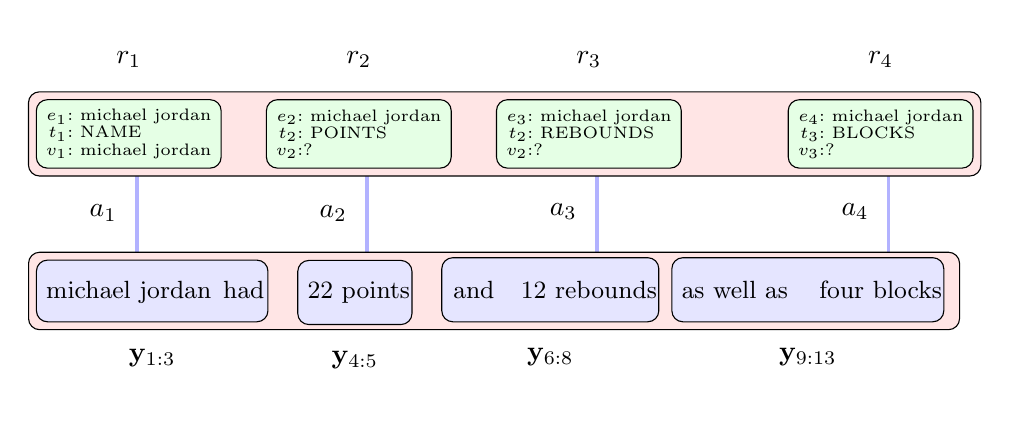
\begin{tikzpicture}[every node/.style={anchor=base,minimum size=8mm}]
    \matrix  (graph) [matrix of nodes, row sep=0.5em,column sep=-0.3em,
    minimum width=0.2em, minimum height=1em, font=\small,ampersand replacement=\&] {
      $\subalign{e_1:& \textrm{ michael jordan}\\ t_1:& \textrm{ NAME}\\ v_1:& \textrm{ michael jordan}}$\&
      \&$\subalign{e_2:& \textrm{ michael jordan}\\ t_2:& \textrm{ POINTS}\\ v_2:& ?}$\&
      \&$\subalign{e_3:& \textrm{ michael jordan}\\ t_2:& \textrm{ REBOUNDS}\\ v_2:& ?}$\&
      \&$\subalign{e_4:& \textrm{ michael jordan}\\ t_3:& \textrm{ BLOCKS}\\ v_3:& ?}$ \\
      \textcolor{white}{a}\& \\
      michael jordan \& had \& % 2
      22 points \& % 3
      and \& % 4
      12 rebounds \& % 5
      as well as \& % 6
      four blocks \\ % 7
   };

    \begin{scope}[on background layer]

    \draw[draw=blue!30, line width=0.5mm] ($(graph-1-1) + (0.1, 0)$) -- node[left] {$a_1$} ($(graph-3-1) + (0.1, 0)$);
    \draw[draw=blue!30, line width=0.5mm] ($(graph-1-3) + (0.1, 0)$) -- node[left] {$a_2$} ($(graph-3-3) + (0.1, 0)$);
    \draw[draw=blue!30, line width=0.5mm] ($(graph-1-5) + (0.1, 0)$) -- node[left] {$a_3$} ($(graph-3-5) + (0.1, 0)$);
    \draw[draw=blue!30, line width=0.5mm] ($(graph-1-7) + (0.1, 0)$) -- node[left] {$a_4$} ($(graph-3-7) + (0.1, 0)$);


    \draw[rounded corners,fill=red!10] ($ (graph-3-1.north west) +(-0.1,0.1)$) rectangle 
    node[yshift=-1cm]{} ($(graph-3-7.south east) +(0.1,-0.1)$ );
    \draw[rounded corners,fill=red!10] ($ (graph-1-1.north west) +(-0.1,0.1)$) rectangle  
    node[yshift=0.8cm]{} ($(graph-1-7.south east) +(0.1,-0.1)$ );

    \draw[rounded corners,fill=green!10] (graph-1-1.north west) rectangle  node[ yshift =0.9cm] {$r_1$} (graph-1-1.south east);
    \draw[rounded corners,fill=green!10] (graph-1-3.north west) rectangle  node[ yshift =0.9cm] {$r_2$} (graph-1-3.south east);
    \draw[rounded corners,fill=green!10] (graph-1-5.north west) rectangle  node[ yshift =0.9cm] {$r_3$} (graph-1-5.south east);
    \draw[rounded corners,fill=green!10] (graph-1-7.north west) rectangle  node[ yshift =0.9cm] {$r_4$} (graph-1-7.south east);

    \draw[rounded corners, fill=blue!10] (graph-3-1.north west) rectangle 
    node[yshift=-0.9cm]{$\by_{1:3}$}  ($(graph-3-2.south east) + (-0.1, 0)$);
    \draw[rounded corners, fill=blue!10] (graph-3-3.north west) rectangle 
    node[yshift=-0.9cm]{$\by_{4:5}$}  ($(graph-3-3.south east) + (-0.1, 0)$);
    \draw[rounded corners, fill=blue!10] (graph-3-4.north west) rectangle 
    node[yshift=-0.9cm]{$\by_{6:8}$}  ($(graph-3-5.south east) + (-0.1, 0)$);
    \draw[rounded corners, fill=blue!10] (graph-3-6.north west) rectangle 
    node[yshift=-0.9cm]{$\by_{9:13}$}  ($(graph-3-7.south east) + (-0.1, 0)$);
    \end{scope}
  \end{tikzpicture}

\caption{An example of our proposed information extraction procedure
with a fixed segmentation.
We aim to infer the missing values in records.
The missing values $v_j$ are predicted independently.
Records $r_i$ are then chosen, and their ordering is given by $\ba_{1:4}$.
Each $a_i$ then generates a sequence of words to describe its record $r_i$.}
\label{fig:d2t}
\end{figure}

As a concrete example, we use the Rotowire dataset \citep{wiseman2017d2t}.
Rotowire contains summaries of basketball games $\by$ aligned with the respective
box scores $\br$ of those games.
Consider the datum in Figure~\ref{fig:d2t} that consists of three records
and the statement $\by = $``michael jordan had 22 points and 12 rebounds as well as four blocks''.
For this example, the process of information extraction is to infer 
the values $\bv$ of the records given the entities $\be$, types $\bt$, and the text $\by$.
We want to infer the value $v_2$ of the second record $r_2$ given 
the entity ``michael jordan'', the type POINTS, as well as the text $\by$.
Conditioning on the whole $\by$ is wasteful as different segments of text
may be referring to different records, so we instead posit that there is a 
latent alignment $\ba$ from words to records.
In this case we have $\by_{4:5}$ are both aligned to and therefore generated by $r_2$.

\paragraph{Proposal}
We propose to verify the efficacy of the LVM framework in the
semi-supervised information extraction setting,
with the following goals:
\begin{enumerate}
\item By formulating a LVM for generating text conditioned on data,
    obtain an information extraction system through posterior inference.
\item Demonstrate strong extractive performance with minimal labels.
\item Move towards a model for knowledge graph completion that captures
    the full joint distribution.
\end{enumerate}
We present one instance of a LVM and outline how it can be used to obtain
an information extraction model without direct supervision,
then argue that the same approach can be applied in even more ambitious settings.
Our proposed LVM is a conditional generative model that specifies
the relationship between data, specifically the entities and types, and text.
We denote this model \texttt{Values}.
%Let $\by$ be the text, $\ba$ be a latent variable that represents the
%alignments from words to records,
%$\bv$ all the values in a datum of records,
%and $\be,\bt$ the entities and types respectively.
Similar to the models defined in \citet{wiseman2018template} and \citet{liang2009semalign},
our model takes the form of a hidden semi-Markov model (HSMM).
The primary difference is that the other models simply assumed the records
were complete and conditioned on them, whereas ours learns to generate the values.
For our model, we have observed $\set{\be,\bt}$ and latent $\set{\bv,\ba}$, 
where $\be$ are the entities, $\bt$ are the types, $\bv$ are the values, and $\ba$ are
record indices.
\texttt{Values} is given by the following generative process:
\begin{enumerate}
\item Prior Value Choice: $p(\bv\mid\be,\bt)$.
For each entity and type pair in our datum of records, we predict a value.
For example, given `michael jordan' and POINTS, we predict 19.
Each value is predicted independently.
\item Prior Record Choice: $p(\ba\mid\bv,\be,\bt) = \prod_i p(a_i\mid a_{i-1},\bv,\be,\bt)$.
Conditioned on our choices of values as well as the given entities and records,
in other words a completed data with no missing values,
we choose a sequence of records $\ba = \set{a_1,\ldots,a_T}$ to describe with a Markov model.
\item Word Choice: $p(\by\mid\ba,\bv,\be,\bt)$.
For each alignment $a_i$,
we choose a sequence of words $\by_i = \set{y_{i1},\ldots,y_{iJ}}$ to describe the record
indicated by the alignment.
With the HSMM formulation, we have that within each segment aligned to a record,
the words are modeled autoregressively.
\end{enumerate}
We obtain an information extraction system by using the 
\textbf{posterior} distribution over alignments and values:
\begin{linenomath*}
$$
p(\ba,\bv\mid\by,\be,\bt)=\frac{p(\by,\ba,\bv\mid\be,\bt)}{p(\by\mid\be,\bt)}
=\frac{p(\by,\ba,\bv\mid\be,\bt)}{\sum_{\ba,\bv} p(\by,\ba,\bv\mid\be,\bt)}.
$$
\end{linenomath*}
Although the HSMM formulation allows the summation (marginalization) over alignments to be carried out efficiently,
we cannot marginalize over value assignments.
We instead resort to variational inference as in \citet{deng2018attn},
where we learn an approximation of the posterior distribution $q(\ba,\bv\mid\by,\be,\bt)$
with a separate model.
% Can marginalize over alignments, so only a partial variational approximation is needed
We can train the conditional generative model and the approximate posterior jointly 
by maximizing a lower bound on the log marginal likelihood of $\by$ with gradient-based methods.
The resulting approximate posterior $q(\ba,\bv\mid\by,\be,\bt)$ can be used independently of the 
generative model as an information extraction system that gives a distribution over
values in a table of records and alignments from text to records.

We will evaluate our approach on the 
TAC KBP 2015 slot filling, TACRED \citep{zhang2017slotfilling},
and ROTOWIRE \citep{wiseman2017d2t} datasets in order to compare to previous work.
The goal will be to demonstrate competitive performance on
extraction metrics such as precision, recall, and F1, while using as little supervision
as possible by ignoring subsets of the given information.
For example, with the model \texttt{Values}, we can allow the model to only learn from
subsets of the given values (or none at all) in ROTOWIRE, such as only
the home team's statistics, at training time.
Given success in that goal, the next step would be to extend the model
to capture more of the joint distribution with the aim of boosting sample and label efficiency.
Possible extensions in this direction include coreference resolution \citep{haghighi2010coref},
learning the types of relations in a semi-supervised manner,
leveraging discourse structure to improve the conditional generative model
\citep{sauper2009wiki}, explicitly modeling nuisance variables such as
author style \citep{hsu2017speech}, and incorporating multi-hop
reasoning in order to leverage relationships between entities
\citep{chen2018diva,rock17prove}.

\begin{comment}
%TODO: Experiments, Evaluation, and Expectations? Also shortcomings? Short paragraph
We will evaluate our initial approach on the Rotowire dataset, and
extensions to our model that will include entity tracking and event resolution on the 
automatic content extraction (ACE) \citep{ace2004} and the Text Analysis Conference's
Streaming Multimedia Knowledge Base Population (SM-KBP) datasets.
We expect the variance of the gradient estimator to be an issue, in particular its
effect on sample complexity. In previous work, we observed that gradient estimators
based on exact inference resulted in better sample complexity than
approximate inference \citep{deng2018attn}, and we expect that controlling the variance 
of the gradient estimator will be of paramount importance for the success of our proposed method.
\end{comment}

Given admittance to the NDSEG Fellowship Program, I will evaluate the application of
LVMs to the problem of information extraction.
As a result of the digital age, the ubiquity of information networks as well as their 
enormous growth makes it clear that a method for training information extraction systems
with minimal supervision is a necessity.
I will push for scalable information extraction systems that require minimal supervision
by recasting information extraction as a generative modeling problem.

%\begin{comment}
\newpage
\section*{Outline}
\begin{enumerate}
\item Introduction
    \begin{enumerate}
    \item Relevance to BAA
        \begin{enumerate}
        \item Intro to information networks and KG
            \begin{enumerate}
            \item Information networks and decision making
            \item Specify knowledge graphs as the information networks we are interested in
            \item Brief outline of knowledge graphs, ie nodes are entities, contain sets of facts,
                edges specify relationships between facts (can include self-loops)
            \end{enumerate}
        \item Argument that KGs cannot be populated by hand. (Brief outline of methods for populating,
            no in-depth descriptions provided in this proposal)
            \begin{enumerate}
            \item Link prediction
            \item Multi-hop link prediction
            \item Corpora-based
            \end{enumerate}
        \item Proposal: train information extraction systems by recasting as a
            generative modeling problem.
        \end{enumerate}
    \item Supervision in Information Extraction
        \begin{enumerate}
        \item Define information extraction
            \begin{enumerate}
            \item The goal is to produce structured representations of information from
                a given unstructured text.
            \item Ideally, but not necessarily computer-readable in addition to human-readable.
            \item A typical pipeline for information extraction includes
                text segmentation, named entity recognition, coreference resolution,
                relation extraction, and finally producing structured representations of the unlabeled text.
            \item This is knowledge-base completion.
            \item We are primarily interested in knowledge-base completion,
                as the other tasks such named entity recognition are typically
                part of a pipeline aimed at knowledge-base completion.
            \end{enumerate}
        \item Argue for LVM approach to unify all parts of the pipeline and train
            end-to-end with minimal supervision.
        \item We aim to unify these two approaches through recently developed techniques for training LVMs
            parameterized with neural networks.
        \end{enumerate}
    \item End-to-end trends and LVMs
        \begin{enumerate}
        \item Draw parallels to progress in translation, mainly in terms of structure?
            \begin{enumerate}
            \item Statistical machine translation: pipelines
            \item End-to-end with Sutskever
            \item Deterministic structure via attention Bahdanau
            \item Latent attention \citet{deng2018attn}
            \end{enumerate}
        \item Leverage modularity of both the neural network and LVM frameworks
            to incorporate more of the pipeline into a joint training framework.
        \item \citet{qu2017ssre} Semi-supervised relation extraction (which is pretty much similar)
            How is what I want different? Capitalize on the progress of powerful generative models,
            can argue that their model is much weaker in terms of generative power,
            but the framework is similar (they perform coordinate ascent in a LVM).
        \end{enumerate}
    \item Recent advances in neural LVMs
        \begin{enumerate}
        \item Semi-supervised LVMs \citet{kingma2014ssvae}?
        \item Demonstrate that parameterization with a neural network does not affect computational
            complexity of inference.
        \item Then the same technique can be applied to model with more structure,
            as long as the graphical model itself permits tractable inference.
        \item In this proposal, we focus on the hidden semi-Markov model (HSMM),
            used in \citet{liang2009semalign} for the task of aligning segments of text to
            records in a knowledge base without supervision. 
        \item As in \citet{liang2009semalign}, we are interested in learning a generative model of text so that
            we can minimize the amount of supervision necessary for training an
            information extraction system.
        \item Also that although worse sample complexity, using an approximate posterior
            with monte carlo sampling achieves comparable performance.
        \end{enumerate}
    \end{enumerate}
\item Background and Notation
    \begin{enumerate}
    \item Formal notation for elements of the dataset
    \item Define the distribution we would like to learn: $p(z\mid y, x)$.
        $z$ and $x$ are placeholders and will change, but $y$ is always the text.
    \item Link to rotowire example
        (argument is that ACE is made up of ontonotes-like sentences, so all short-form)
    \item Clarify that the scope of posterior inference is very general.
    \end{enumerate}
\item Proposal
    \begin{enumerate}
    \item Outline approach
        \begin{enumerate}
        \item Choose a subset of available data as conditioning,
            and thus it is not modelled.
        \item The joint distribution of the remaining variables,
            both observed and unobserved, will be modelled.
        \end{enumerate}
    \item Link back to motivation. We want to scale information extraction
        by requiring less supervision.
    \item We present one model as an example, which we will serve as
        a starting point for the proposed research.
    \item Define generative model: HSMM as in \citep{liang2009semalign},
        and \citep{wiseman2018template}.
        The generative story (a picture would be helpful):
        \begin{enumerate}
        \item Fill in values
        \item Choose alignments
        \item Choose words
        \end{enumerate}
    \item Define IE as the distribution we would like to learn
        \begin{enumerate}
        %\item Align: $p(c\mid\by,\br)$
        \item Values: $p(c,\bv\mid\by,\be,\bt)$ (Just this one)
        %\item ??: $p()$
        \end{enumerate}
    \item We either use the posterior distribution of the conditional model
        or learn an approximation of it.
    \item Training and Inference
        \begin{enumerate}
        \item As we are dealing with large state spaces,
            we train with an approximate posterior in order to satisfy memory constraints.
        \item Highlight that the approx posterior is a SEPARATE model
            that can be used completely independently from generative model,
            i.e. we throw away generative model after training.
        \item We maximize a lower bound on the log marginal likelihood,
            called the evidence lower bound.
        \end{enumerate}
    \item Experiments, evaluation, and expectation
        \begin{enumerate}
        \item Evaluate on Rotowire.
        \item We evaluate \texttt{Values} using the precision, recall, and F1 score on the task
            of predicting the values associated with entities, otherwise known as slot-filling.
        \item What would success look like?
            \begin{enumerate}
            \item Competitive to supervised methods when supervision is available
            \item But able to be applied when supervision is not available
            \item Able to leverage lots of unlabeled data during training,
                and success would see a marked improvement over purely supervised methods
                as well as the purely supervised version of this model.
            \item Would provide explanations for the answers (ie segmentations).
            \end{enumerate}
        \item Also on ACE?
        \end{enumerate}
    \item Future work
        \begin{enumerate}
        \item Incorporate more structure into the generative model,
            for example entity tracking or coreference resolution \citet{haghighi2010coref}.
        \item Model more structure in the data, for example the edges between nodes
            in the knowledge graph \citet{chen2018diva}.
        \item `Multi-hop' reasoning, where we try to compose relationships to infer new ones,
            i.e. through unification \citet{chen2018diva,rock17prove}.
        \end{enumerate}
    \item Conclusion
        \begin{enumerate}
        \item Please accept!
        \item Recap: Minimal supervision IE systems so that they can scale to
            extracting information for large information networks from large bodies of text.
        \end{enumerate}
    \end{enumerate}
\end{enumerate}
%\end{comment}

\newpage
\bibliographystyle{plainnat}
\bibliography{w}

\end{document}

